\documentclass{standalone}
\usepackage{tikz}
%------------tikz Setup------------

\tikzstyle{ball} = [circle,shading=ball, ball color=black,
    minimum size=1mm,inner sep=1.3pt]
\tikzstyle{miniball} = [circle,shading=ball, ball color=black,
    minimum size=1mm,inner sep=0.5pt]
\tikzstyle{mminiball} = [circle,shading=ball, ball color=black,
    minimum size=0.6mm,inner sep=0.1pt]
\usetikzlibrary{arrows.meta}
\usetikzlibrary{angles, quotes}
\tikzset{>={Latex[length=2mm,width=1.5mm]}}
\tikzset{->-/.style={decoration={markings, mark=at position #1 with
  {\arrow{>}}},postaction={decorate}}}
\usetikzlibrary{decorations.pathmorphing}
\usetikzlibrary{decorations.pathreplacing}
\usetikzlibrary{arrows.meta,calc}
\usetikzlibrary{bending}
\usetikzlibrary{decorations.markings,shapes.geometric}
\tikzset{->-/.style={decoration={markings, mark=at position #1 with
  {\arrow{>}}},postaction={decorate}}}
\tikzset{-|-/.style={decoration={markings, mark=at position #1 with
  {\arrow{stealth}}},postaction={decorate}}}
\tikzset{movearrow/.style 2 args ={
        decoration={markings,
    mark= at position {#1} with {\arrow{#2}} ,
        },
        postaction={decorate}
    }
}


\begin{document}
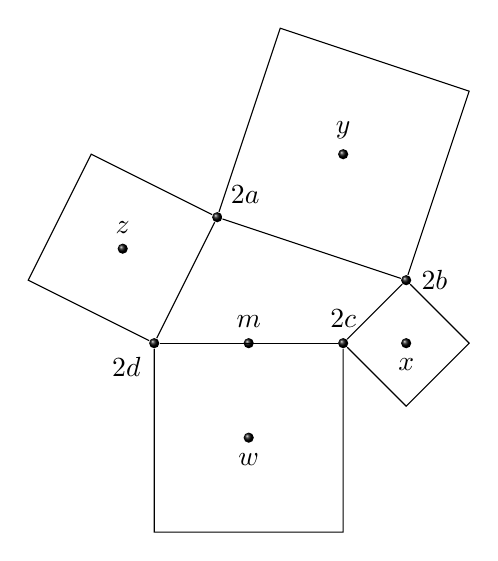
\begin{tikzpicture}
\begin{scope}[scale=0.4]
    %vertices
    \node[ball, label={above right:$2a$}] (A) at (-1,3) {};
    \node[ball, label={right:$2b$}] (B) at (5,1) {};
    \node[ball, label={$2c$}] (C) at (3,-1) {};
    \node[ball, label={below left:$2d$}] (D) at (-3,-1) {};
    %midpoint
    \node[ball, label={above:$m$}] (m) at (0,-1) {};
    %centers
    \node[ball, label={below:$w$}] (w) at (0,-4) {};
    \node[ball, label={below:$x$}] (x) at (5,-1) {};
    \node[ball, label={above:$y$}] (y) at (3,5) {};
    \node[ball, label={above:$z$}] (z) at (-4,2) {};
    %squares
    \draw (A) -- (1,9) -- (7,7) -- (B);
    \draw (D) -- (-7,1) -- (-5,5) -- (A);
    \draw (B) -- (7,-1) -- (5,-3) -- (C);
    \draw (C) -- (3,-7) -- (-3,-7) -- (D);
    %quadrilateral 
    \draw (A) to (B);
    \draw (B) to (C);
    \draw (C) to (D);
    \draw (D) to (A);
\end{scope}
\end{tikzpicture}
\end{document}